% Options for packages loaded elsewhere
\PassOptionsToPackage{unicode}{hyperref}
\PassOptionsToPackage{hyphens}{url}
%
\documentclass[
]{book}
\usepackage{lmodern}
\usepackage{amssymb,amsmath}
\usepackage{ifxetex,ifluatex}
\ifnum 0\ifxetex 1\fi\ifluatex 1\fi=0 % if pdftex
  \usepackage[T1]{fontenc}
  \usepackage[utf8]{inputenc}
  \usepackage{textcomp} % provide euro and other symbols
\else % if luatex or xetex
  \usepackage{unicode-math}
  \defaultfontfeatures{Scale=MatchLowercase}
  \defaultfontfeatures[\rmfamily]{Ligatures=TeX,Scale=1}
\fi
% Use upquote if available, for straight quotes in verbatim environments
\IfFileExists{upquote.sty}{\usepackage{upquote}}{}
\IfFileExists{microtype.sty}{% use microtype if available
  \usepackage[]{microtype}
  \UseMicrotypeSet[protrusion]{basicmath} % disable protrusion for tt fonts
}{}
\makeatletter
\@ifundefined{KOMAClassName}{% if non-KOMA class
  \IfFileExists{parskip.sty}{%
    \usepackage{parskip}
  }{% else
    \setlength{\parindent}{0pt}
    \setlength{\parskip}{6pt plus 2pt minus 1pt}}
}{% if KOMA class
  \KOMAoptions{parskip=half}}
\makeatother
\usepackage{xcolor}
\IfFileExists{xurl.sty}{\usepackage{xurl}}{} % add URL line breaks if available
\IfFileExists{bookmark.sty}{\usepackage{bookmark}}{\usepackage{hyperref}}
\hypersetup{
  pdftitle={Urbanization},
  pdfauthor={Dyrehaugen Web Notebook},
  hidelinks,
  pdfcreator={LaTeX via pandoc}}
\urlstyle{same} % disable monospaced font for URLs
\usepackage{longtable,booktabs}
% Correct order of tables after \paragraph or \subparagraph
\usepackage{etoolbox}
\makeatletter
\patchcmd\longtable{\par}{\if@noskipsec\mbox{}\fi\par}{}{}
\makeatother
% Allow footnotes in longtable head/foot
\IfFileExists{footnotehyper.sty}{\usepackage{footnotehyper}}{\usepackage{footnote}}
\makesavenoteenv{longtable}
\usepackage{graphicx}
\makeatletter
\def\maxwidth{\ifdim\Gin@nat@width>\linewidth\linewidth\else\Gin@nat@width\fi}
\def\maxheight{\ifdim\Gin@nat@height>\textheight\textheight\else\Gin@nat@height\fi}
\makeatother
% Scale images if necessary, so that they will not overflow the page
% margins by default, and it is still possible to overwrite the defaults
% using explicit options in \includegraphics[width, height, ...]{}
\setkeys{Gin}{width=\maxwidth,height=\maxheight,keepaspectratio}
% Set default figure placement to htbp
\makeatletter
\def\fps@figure{htbp}
\makeatother
\setlength{\emergencystretch}{3em} % prevent overfull lines
\providecommand{\tightlist}{%
  \setlength{\itemsep}{0pt}\setlength{\parskip}{0pt}}
\setcounter{secnumdepth}{5}
\usepackage{booktabs}
\usepackage{amsthm}
\makeatletter
\def\thm@space@setup{%
  \thm@preskip=8pt plus 2pt minus 4pt
  \thm@postskip=\thm@preskip
}
\makeatother

\renewcommand\chaptername{}
\usepackage[]{natbib}
\bibliographystyle{apalike}

\title{Urbanization}
\author{Dyrehaugen Web Notebook}
\date{2021-11-02}

\begin{document}
\maketitle

{
\setcounter{tocdepth}{1}
\tableofcontents
}
\hypertarget{urbanization}{%
\chapter{Urbanization}\label{urbanization}}

Web Collection - Work in Progress


\includegraphics{fig/zelda.jpg}

\emph{Urban Scaling} is about non-linear relationships stemming from agglomeration of humans
in geographic space.

Recently the \emph{Corona virus COVID-19} has hit - overproportionally in densely populated urban areas.
\emph{Urban Epidemics} is an example of \emph{Urban Scaling}.

Urban Scaling can be positive - \emph{agglomeration economics of scale} - or negative
\emph{agglomeration diseconomics of scale} - like the corona urban epidemic.

As motivation we take this 3D map of the Coronavirus (Covid-19) outbreak in the US.

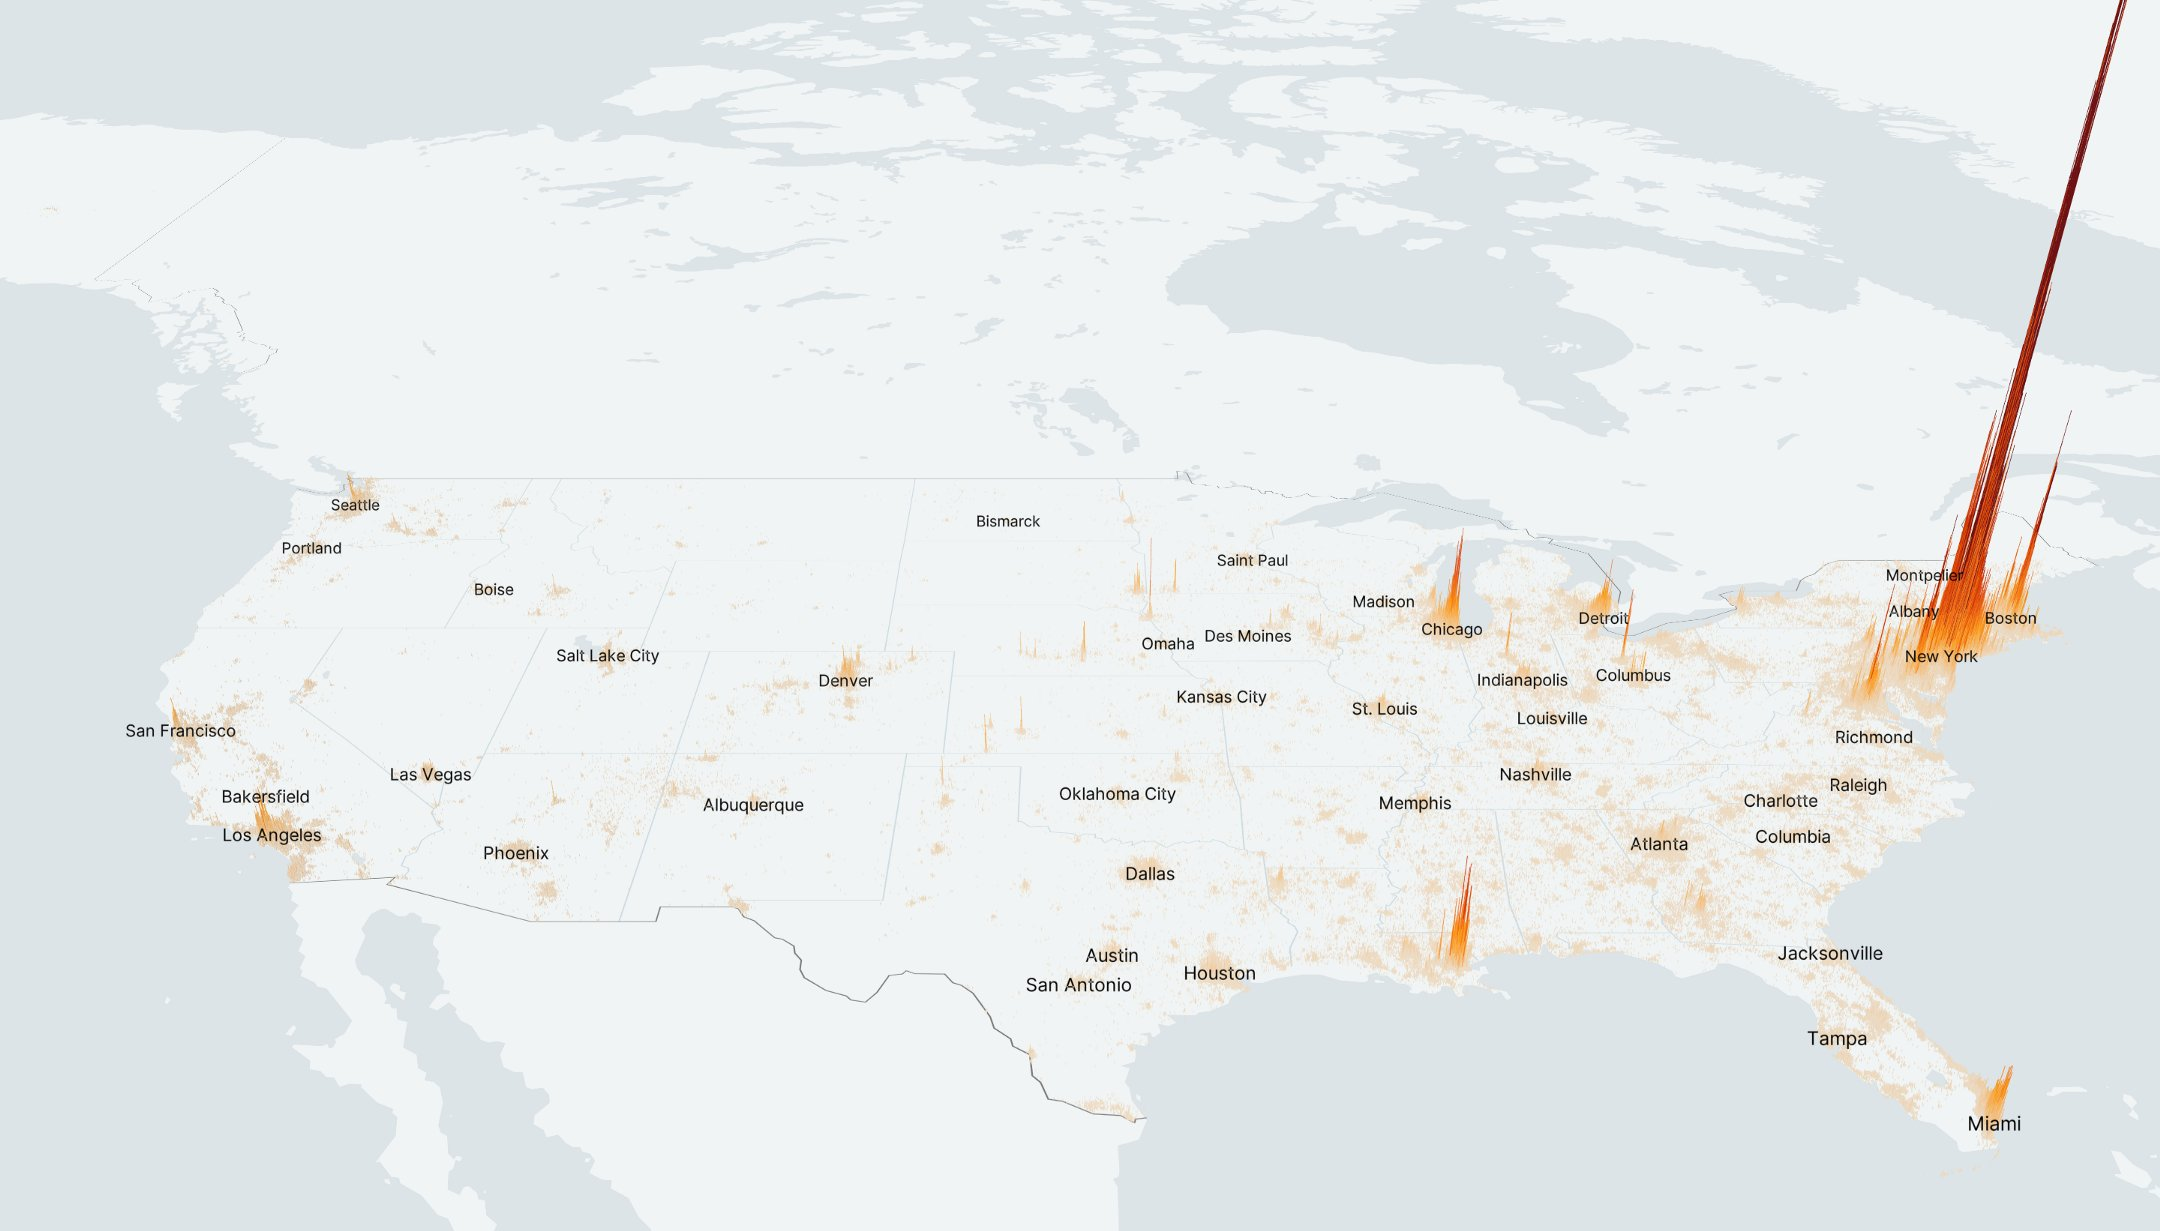
\includegraphics{fig/Corona_Cases_pc_US_3D.jpeg}

Fig. 1 Confirmed Corona Cases per Population in US Counties May 2020 (Source: \citep[ medium.com]{topos_ai}(\url{https://medium.com/topos-ai/visualizing-covid-19-beyond-counties-d1026e5c7efa}) )

\emph{Urban Epidemics} is a particular variant of \emph{Urban Scaling}.

\hypertarget{urban-degrowth}{%
\chapter{Urban Degrowth}\label{urban-degrowth}}

\hypertarget{imaginary-urban-downscaling---exiting-the-economy}{%
\section{Imaginary: Urban Downscaling - Exiting the Economy}\label{imaginary-urban-downscaling---exiting-the-economy}}

\emph{Memo Mastini:}

Decommodifying essential services is also a way for breaking the `productivist nexus' (the twin societal goal of full-time employment and perpetual growth) and, therefore, beginning to downscale the metabolism of our economic system. Imagine if we were to even just partially decommodify the housing stock by expanding public housing and capping the price of private housing at half its present level. Citizens would suddenly be able to work and earn significantly less than they presently do without any loss to their quality of life. The economy would produce less as a result, but it would also need much less. In such an economy private wealth (or GDP) may shrink reducing the incomes of corporations and the very rich, but public wealth would increase, significantly improving the lives of everyone else. And given the overwhelming scientific evidence on the limits of decoupling GDP growth from environmental impacts, this is the only way to meet our climate commitments.

\href{https://www.slu.se/en/Collaborative-Centres-and-Projects/slu-urban-future/activities/urban-readings/housing-for-a-socio-ecological-transformation/}{Mastini}

\emph{Memo Savini:}

A systemic imaginary of transition,
degrowth is a `source of hope and dreams'
for a more equitable and sustainable society
that has `exited the economy'.

Outlines three transitions toward urban degrowth,
arguing for a regional imaginary of polycentric autonomism,
a paradigm of finity in development,
and care for habitability as principle of spatial organization.

A degrowth perspective couples the critique of contemporary
market economies with the prefiguration of a society
emancipated from the imperative of competition.

A degrowth imaginary begins from evidence indicating
the impossibility of decoupling
economic growth from environmental destruction

Against the hegemony of growth in (eco)modernist thinking, degrowers call for a de-
commodification of nature, labour, land, and housing and for an ethic of solidarity, coop-
eration, and wellbeing.

Against consumerism - a
cultural shift toward values of buen vivir, sufficiency, and simplicity

In sum, degrowth is a project of transitioning systematically
toward a new society.

First, the paper argues for an imaginary of regions as polycentric federations of
autonomous settlements. Second, it calls for a planning paradigm led by principles of finity
in urban development. Third, it proposes to mobilize the notion of habitability in shaping of
socio-spatial relations.

Rethink cities as dynamic sites of deceleration, regeneration, and redistribution.

Urban degrowth research has largely demonstrated the capacity of real-life
practices of urban dwelling to plant the seeds of a more
cooperative, symbiotic and democratic urban society.

\href{https://journals.sagepub.com/doi/10.1177/0308518X20981391}{Savini}
\href{/pdf/Savini_2020_Urban_Degrowth.pdf}{(pdf)}

\hypertarget{urban-energy-use}{%
\section{Urban Energy Use}\label{urban-energy-use}}

\emph{Fix (twitter)}

Are cities sustainable? A loaded question, yes. But one we should think about nonetheless.
Here's an undeniable fact: urbanization correlates strongly with energy use per person.

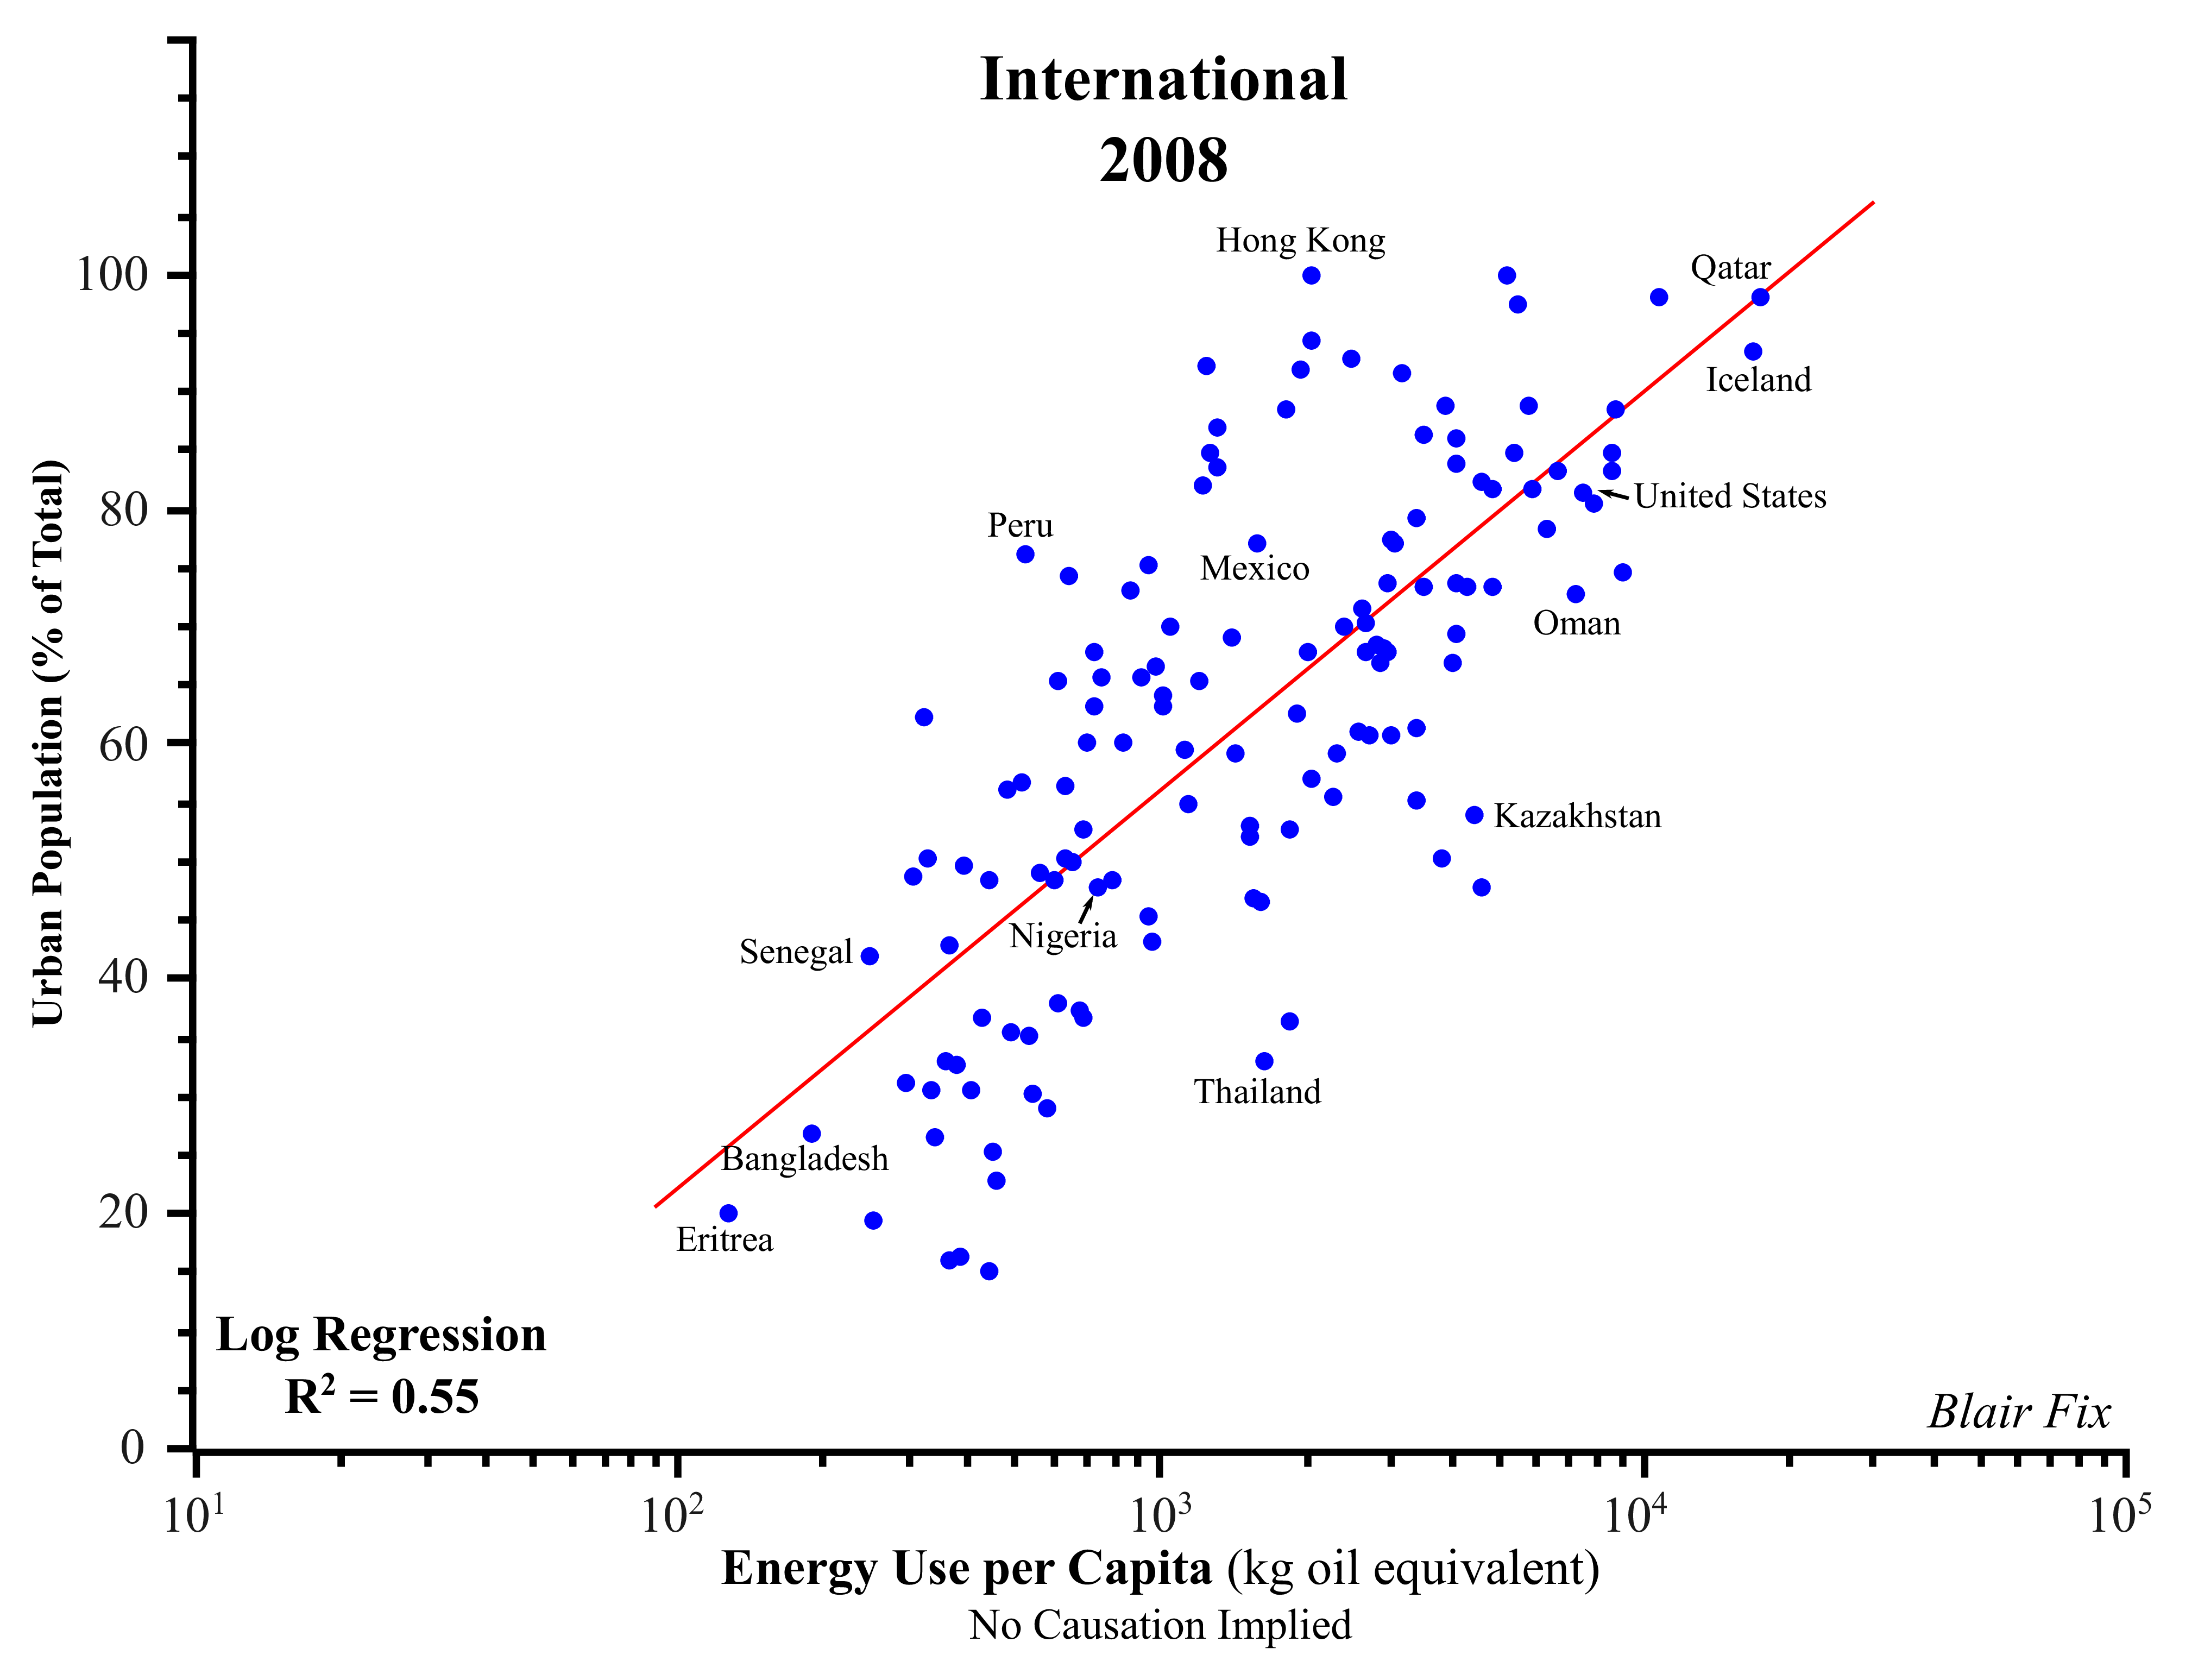
\includegraphics{fig/Fix_2008_Urban_Energy_Use.png}

\hypertarget{urban-epidemics}{%
\chapter{Urban Epidemics}\label{urban-epidemics}}

\textbf{Social Distancing} has become the mantra of policy response to the 2020 \emph{Corona Outbreak}.
Economic forces have for centruries pushed people closer and closer together in urban agglomerations.
The emergence of a major \emph{pandemic} in the 21th century - although forewarned - obviously was not
a risk factor considered seriously by these same \emph{economic forces} - neither private nor public
\emph{decisionmakers} when promoting and allowing the construction of the great agglomerations.

\emph{Homo Sapiens} was not made by nature to live in megacities.
The corona outbreak is a piece of nature striking back as a reminder of the vulnerability of
the artificial urban environment to the most basic of natural evolution - mutation of a virus.

\href{https://arxiv.org/abs/2003.10376}{\emph{Stier (2020)}} provides an empirical treatment of the relation between
urban size and the speed of epidemic spread in the US during the 2020 corona outbreak.
The main findings are:

\begin{itemize}
\item
  \emph{faster} spreading in larger cities
\item
  \emph{larger} fractions of the population infected
\item
  \emph{more aggresive} distancing needed
\end{itemize}

The virus is new, i.e.~\emph{everyone is susceptible}.
The virus provokes a respiratory disease which makes \emph{transmission easy}.
The reproductive number \(R_{eff}\) seems to be higher than for ordinary influenza.
Two factors determine how contagious the disease is: 1)length of the infectious period
and 2) social contact intensity.
Cities are the best breeding ground due to the high contact intensity.

\begin{quote}
The higher socioeconomic connectivity of larger cities in a fast urbanizing world makes
containing emergent epidemics harder. But the density of socioeconomic connections in cities
can also facilitate the spread of information, social coordination, and innovations necessary to
stop the spread of COVID-19. This information and associated actions can easily spread much
faster than the biological viral contagion. To fight an exponential, we need to create an even
faster exponential! (\emph{Stier (2020)})
\end{quote}

So - the fight between \emph{Humans} and \emph{Nature} goes on!
The bigger question - of course - being whether Humans should consider stopping creating such
large {[}\emph{unhuman}{]} agglomerations. There are many \emph{diseconomics to scale} - epidemics being just one.
Cities grow due to dominant \emph{economics of scale} -i.e.~benefitting the rich and powerful.
The diseconomics are borne by others. Changing the current path does not seem easy -
it goes to the core issue of \emph{Capitalism}. This is treated \href{https://dyrehaugen.github.io/jdt/cap_urbanisation.html\#the-urban-dimension}{\emph{elsewhere}}.
Here we look into the more narrow theme of
\href{/docs/03-urban-scaling}{Urban Scaling}

\hypertarget{urban-risk}{%
\chapter{Urban Risk}\label{urban-risk}}

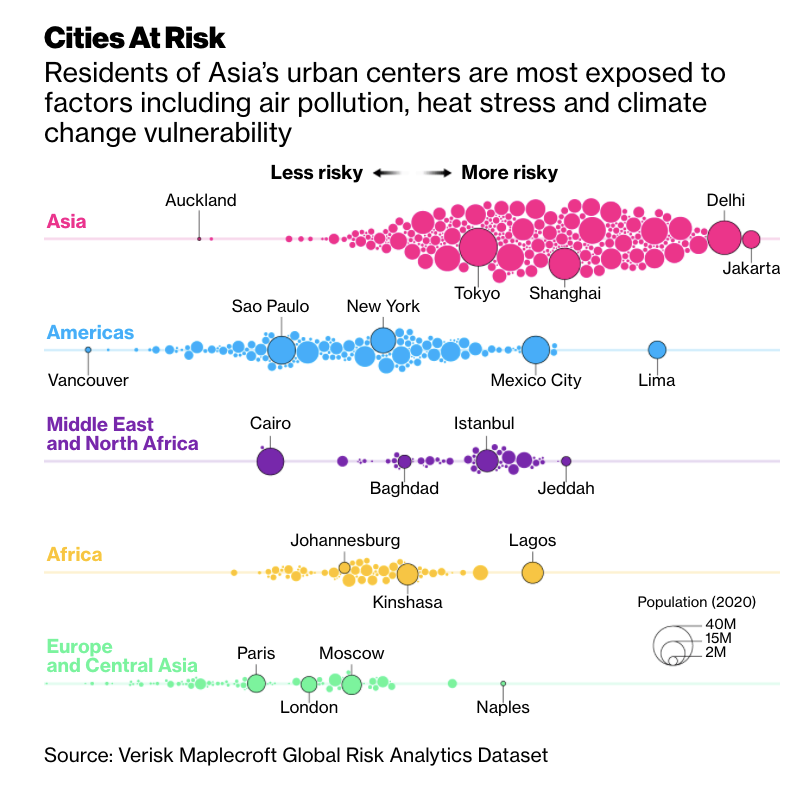
\includegraphics{fig/urban_risk.png}

\href{https://www.bloomberg.com/news/articles/2021-05-12/asian-cities-face-greatest-environmental-risks-report-shows}{Bloomberg (paywall)}

\hypertarget{urban-scaling}{%
\chapter{Urban Scaling}\label{urban-scaling}}

\hypertarget{settlement-size-scaling}{%
\section{Settlement-Size Scaling}\label{settlement-size-scaling}}

\hypertarget{prehistoric}{%
\subsection{Prehistoric}\label{prehistoric}}

\emph{Haas}

Settlement size predicts extreme variation in the rates and magnitudes of many social and ecological processes in human societies. Yet, the factors that drive human settlement-size variation remain poorly understood. Size variation among economically integrated settlements tends to be heavy tailed such that the smallest settlements are extremely common and the largest settlements extremely large and rare. The upper tail of this size distribution is often formalized mathematically as a power-law function. Explanations for this scaling structure in human settlement systems tend to emphasize complex socioeconomic processes including agriculture, manufacturing, and warfare---behaviors that tend to differentially nucleate and disperse populations hierarchically among settlements. But, the degree to which heavy-tailed settlement-size variation requires such complex behaviors remains unclear. By examining the settlement patterns of eight prehistoric New World hunter-gatherer settlement systems spanning three distinct environmental contexts, this analysis explores the degree to which heavy-tailed settlement-size scaling depends on the aforementioned socioeconomic complexities. Surprisingly, the analysis finds that power-law models offer plausible and parsimonious statistical descriptions of prehistoric hunter-gatherer settlement-size variation. This finding reveals that incipient forms of hierarchical settlement structure may have preceded socioeconomic complexity in human societies and points to a need for additional research to explicate how mobile foragers came to exhibit settlement patterns that are more commonly associated with hierarchical organization. We propose that hunter-gatherer mobility with preferential attachment to previously occupied locations may account for the observed structure in site-size variation.

\href{https://journals.plos.org/plosone/article?id=10.1371/journal.pone.0140127}{Haas}
\href{pdf/Haas_2015_Prehistoric_Settlement_Size_Scaling.pdf}{(pdf)}

\hypertarget{scaling-laws---to-the-better-or-to-the-worse}{%
\section{Scaling Laws - to the better or to the worse?}\label{scaling-laws---to-the-better-or-to-the-worse}}

``Scaling laws are power-law relationships of the form \(Y = cX^β\), where \(Y\) represents a
variable which varies in a systematic way with the size \(X\) of subsystems and \(c\) and \(β\) are
parameters. They have two powerful advantages: they summarize structural features of
systems in a very efficient way, and they reveal the effect of universal constraints acting
on the structure and development over several orders of magnitude in these systems\ldots{}
The main resources enabling urban
development are the technical and cultural innovations which increase the productivity,
the diversity and the cohesion of human activities; the availability of these resources
relies on the production and exchanges of information \ldots{}
The role of cities as centers for the integration of human capital and as incubators
of invention was rediscovered by the ``new'' economic growth theory, which posits that
knowledge spillovers among individuals and firms are the necessary underpinnings of
growth (Lucas 1988, Romer 1986) \ldots{}
This seemingly spontaneous
process, whereby knowledge produces growth and growth attracts knowledge, is the
engine by which urban centers sustain their development through unfolding innovation.
The essential role of knowledge generation, recombination and circulation within and
across urban areas must be at the core of any proposed explanation for urban scaling."
\href{https://journals.openedition.org/cybergeo/2519}{(Pumain 2006)}

There are however, other more critical views on the story of urban agglomeration.
\href{https://www.citymetric.com/horizons/urbanisation-not-natural-or-inevitable-its-being-inflicted-upon-us-forces-capitalism-900}{Naik and Oldfield (2015) Urbanisation inflicted by Capitalism}
Urbanization is seen as a an enterprise of \emph{The Urban Industry} - a term for the
`interlinked and interdependent relationships among NGOs, academia, business, high culture and governments' that keeps afloat the story of `cities as centers of innovation, creativity, happiness, good health and, even astonishingly the cause and the solution for global warming'. Naik and Oldfield
present evidence to the quite contrary: `cities are in fact creators, incubators and perpetuators of poverty and inequality.' Actually, as they say: `The urbanisation of the world should not be celebrated'.

\hypertarget{scaling-math}{%
\section{Scaling Math}\label{scaling-math}}

Urban Scaling Research finds that Social Contact Intensity is linked to City Size approximately
as a power law:

\(k(N) = k_{0} N^β\)

with β = 1 + δ and δ ≈ 1/6 acording to \href{https://science.sciencemag.org/content/340/6139/1438}{Bettencourt}.

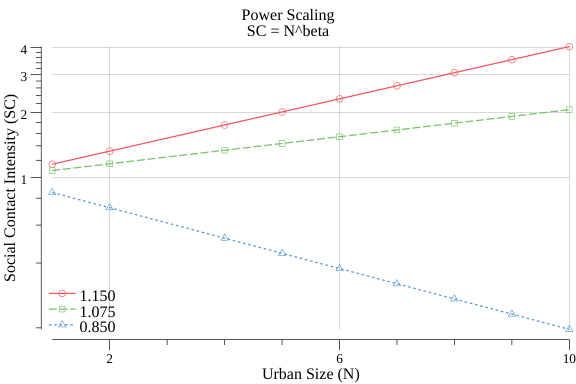
\includegraphics{fig/scale_log.png}

Fig 2. Power Law of Urban Scaling

Fig 2 illustrates the power of scaling. The red line has δ = 0.15 and the green half of this,
δ = 0.075. Both are cases of \emph{positive} or \emph{superlinear} scaling. For comparion δ can also be
negative (sublinear), i.e.larger cities have smaller effects,
as illustrated on the figure with δ = 0.85 (blue line).

A scaling factor of δ = 0.15 is fairly strong: An urban area with 5 times the population -
1 million people compared to another with 200.000 people - has the double Social Contact Intensity.
10 times the population (2 million people) gives 4 times the intensity.

`Social Contact Intensity' - as we use it here - is an umbrella term.
Many aspects of social and economic activity within urban areas will follow such power laws.
Many empirical studies find power laws with β around 1.1 - 1.2 as a general charcteristic.
As Bettencourt puts it: `Cities primary function is open-ended social reactors\ldots{}
{[}which{]} exist in similar, but changing forms over a huge range of scales\ldots{}
{[}and{]} evolve acording to a small set of principles that operate locally\ldots{}
{[}so that{]} the average social, spatial, and infrastructural properties of cities\ldots{}
{[}follow{]} scaling relations that apply to all urban systems.' .

\hypertarget{urban-catastrophes}{%
\section{Urban Catastrophes}\label{urban-catastrophes}}

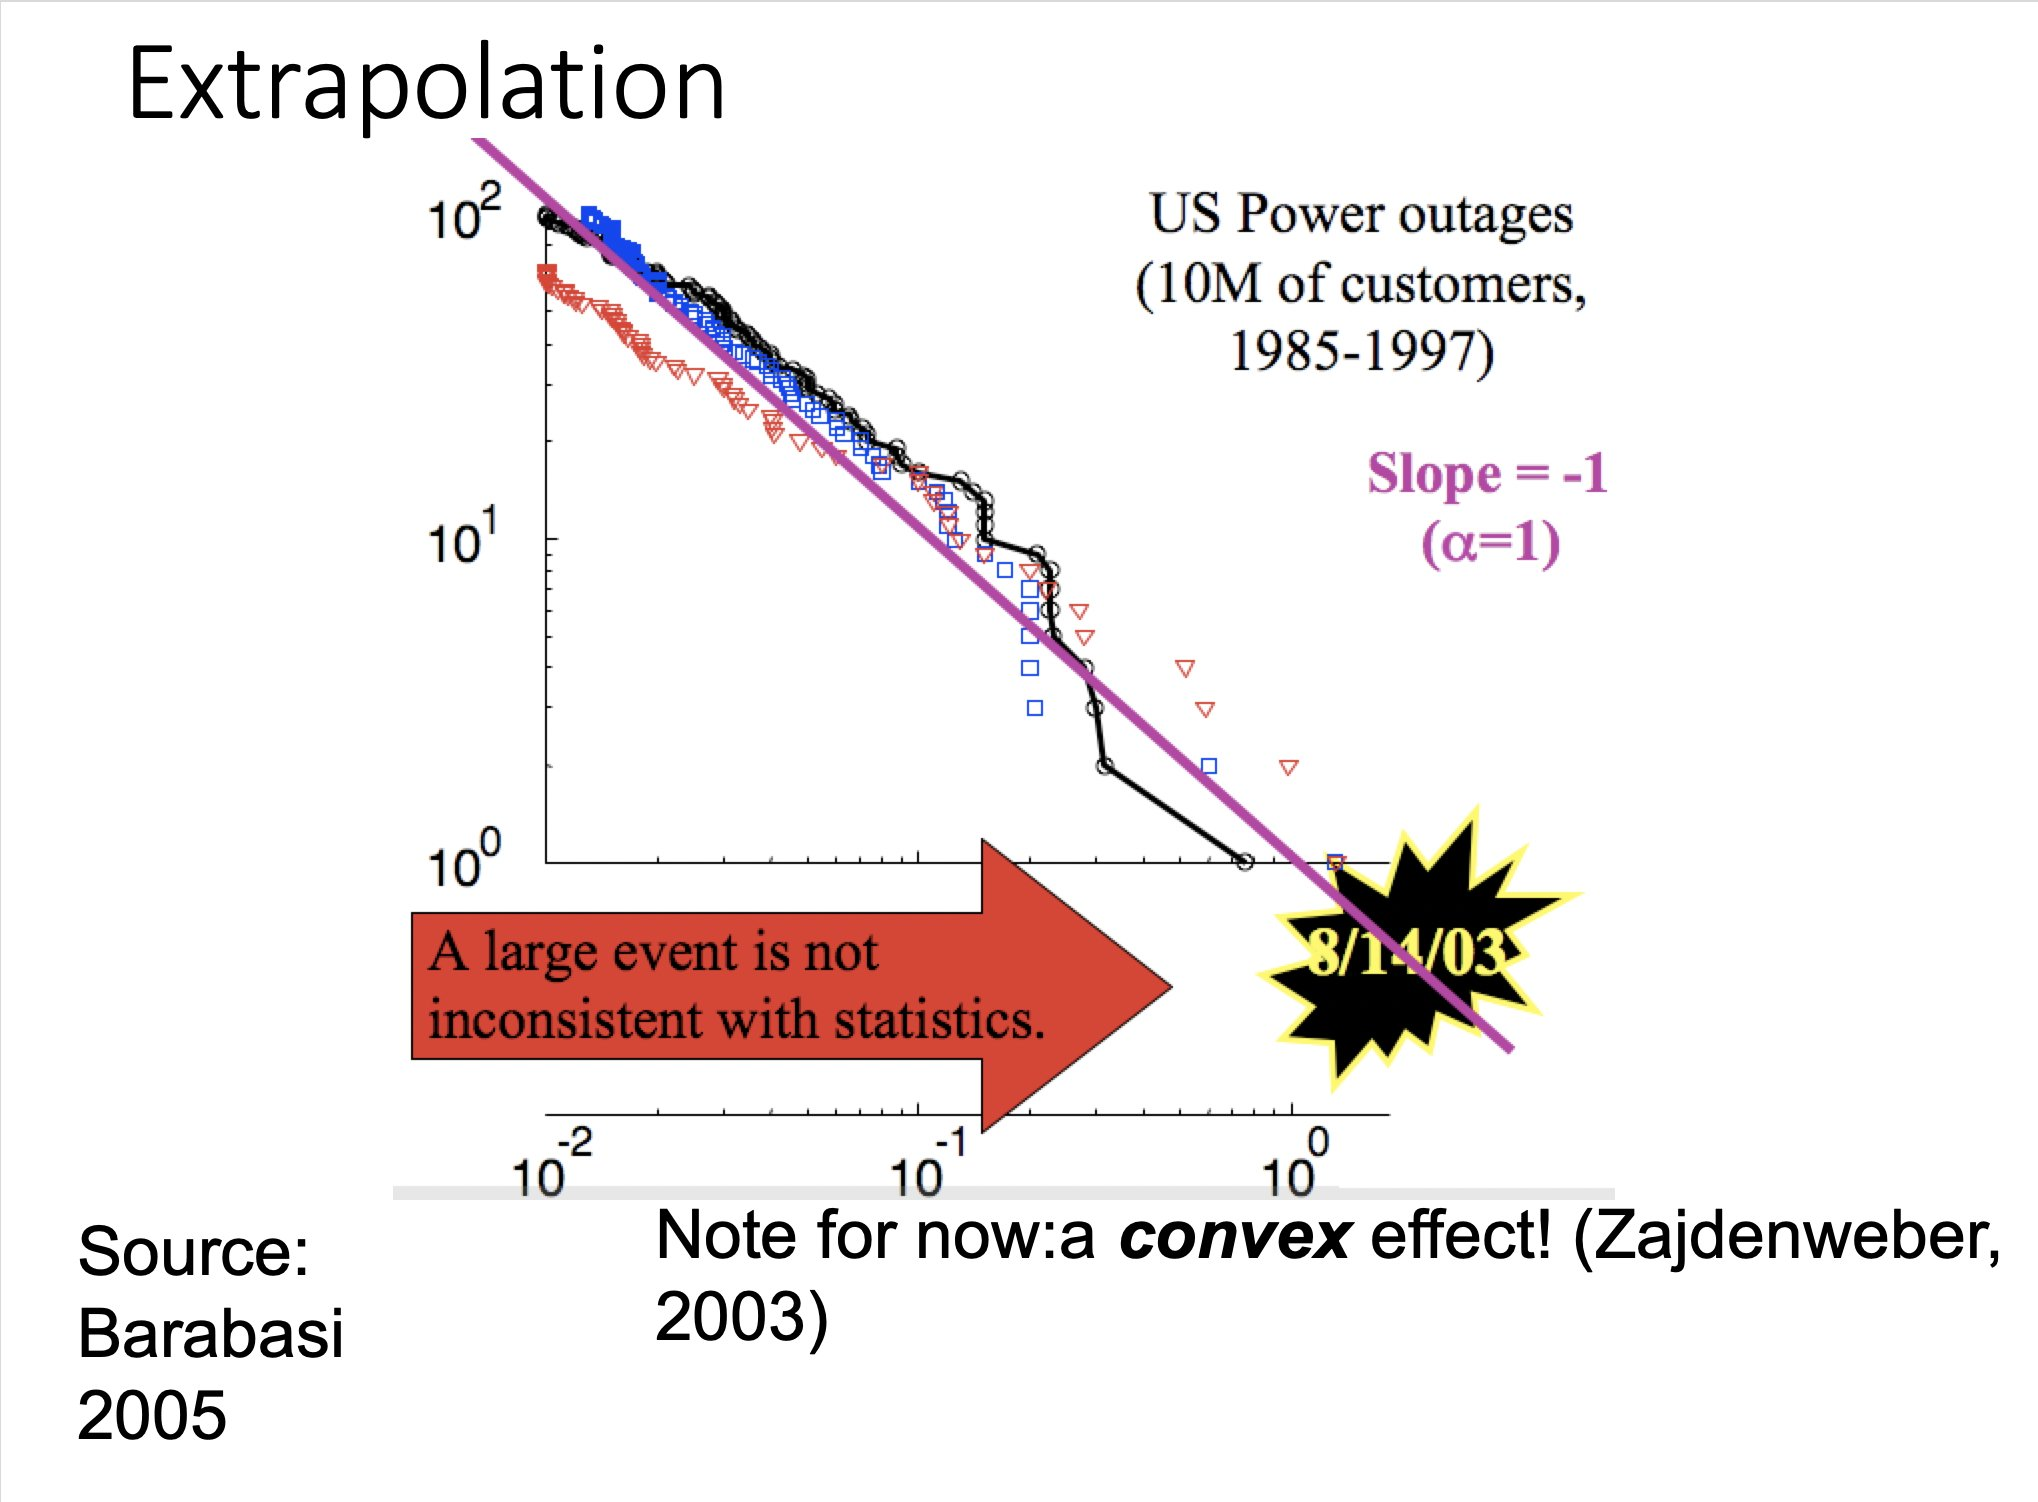
\includegraphics{fig/US_Power_Outages.jpeg}

The probabilities of electricity blackouts may be influenced by the sizes of cities
more than by the details of power grids.

Electric power blackouts can occur on all scales, from local outages to country-wide failures. The probability of a given event depends on the size of the region it affects, according to a mathematical relationship called a power law. The reason for the power law hasn't been clear, but a new model suggests that it results from the same kind of distribution in the sizes of cities {[}1{]}. The model's creators say that understanding the factors that influence blackout probabilities could help engineers make electricity grids more robust.

\href{https://physics.aps.org/articles/v13/122}{Ball (2020) City Size Blackouts}

\href{https://journals.aps.org/prl/abstract/10.1103/PhysRevLett.125.058301}{Nesti (2020) Emergence of Scale-Free Blackout Sizes in Power Grids (PayWall)}

\hypertarget{the-urban-organism}{%
\chapter{The Urban Organism}\label{the-urban-organism}}

\href{https://capitalaspower.com/casp-forum/topic/questions-regarding-mumfords-theory-of-the-mega-machine/\#post-245381}{Mumford' Mega-Machine Theory}

\hypertarget{density}{%
\chapter{Density}\label{density}}

\emph{Density is not the enemy}

\begin{verbatim}
Vertical, centralized density = bad
Broad, decentralized human scaled density = good
No one wants blade runner cities
(twitter)
\end{verbatim}

\hypertarget{high-rise-building}{%
\chapter{High Rise Building}\label{high-rise-building}}

\hypertarget{technological-hurdles}{%
\section{Technological Hurdles}\label{technological-hurdles}}

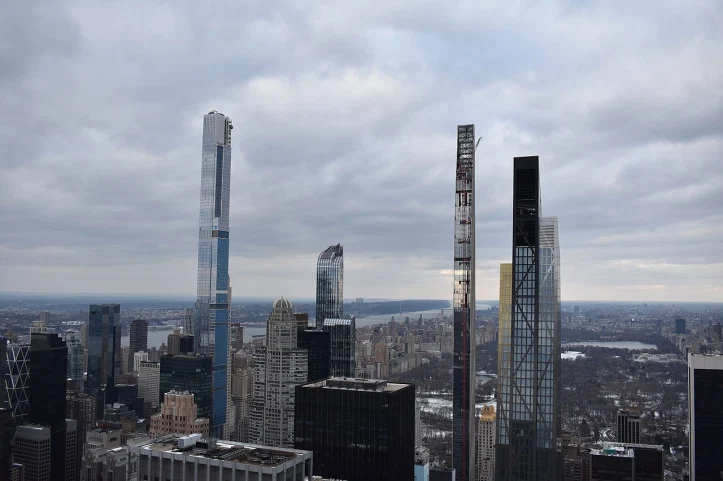
\includegraphics{fig/billionaires_row_2020.png}
Swinging in the Wind: Billionaire's Row \emph{Source:} \href{https://commons.wikimedia.org/wiki/File:Billionaires\%27_Row_2020.jpg}{Wikipedia}

The nearly 1,400-foot tower at 432 Park Avenue, briefly the tallest residential building in the world, was the pinnacle of New York's luxury condo boom half a decade ago, fueled largely by foreign buyers seeking discretion and big returns.

Six years later, residents of the exclusive tower are now at odds with the developers, and each other, making clear that even multimillion-dollar price tags do not guarantee problem-free living. The claims include millions of dollars of water damage from plumbing and mechanical issues; frequent elevator malfunctions; and walls that creak like the galley of a ship --- all of which may be connected to the building's main selling point: its immense height.

Less than a decade after a spate of record-breaking condo towers reached new heights in New York
concerns are raised that some of the construction methods and materials used
have not lived up to the engineering breakthroughs that only recently
enabled 1,000-foot-high trophy apartments.
All buildings sway in the wind, but at exceptional heights, those forces are stronger.

Billionaire's Row is a stretch of supertall towers near Central Park that redefined the city skyline,
and where the identities of virtually all the buyers were concealed by shell companies.

\href{https://www.nytimes.com/2021/02/03/realestate/luxury-high-rise-432-park.html}{NY Times}

\hypertarget{human-settlements}{%
\chapter{Human Settlements}\label{human-settlements}}

\hypertarget{organization-of-life}{%
\section{Organization of Life}\label{organization-of-life}}

Life consists of units within units. In the biological world, we have genes, individuals, groups, species, and ecosystems -- all nested within the biosphere. In the human world, we have genes, individuals, families, villages and cities, provinces, and nations -- all nested within the global village. In both worlds, a problem lurks at every rung of the ladder: a potential conflict between the interests of the lower-level units and the welfare of the higher-level units. What's good for me can be bad for my family. What's good for my family can be bad for my village, and so on, all the way up to what's good for my nation can be bad for the global village.

For most of human existence, until a scant 10 or 15 thousand years ago, the human ladder was truncated. All groups were small groups whose members knew each other as individuals. These groups were loosely organized into tribes of a few thousand people, but cities, provinces, and nations were unknown.

Today, over half the earth's population resides in cities and the most populous nations teem with billions of people, but groups the size of villages still deserve a special status. They are the social units that we are genetically adapted to live within and they can provide a blueprint for larger social units, including the largest of them all -- the global village of nations.

Every once in a great while, the good manage to decisively suppress selfishness within their ranks. Then something extraordinary happens. The group becomes a higher-level organism.

The idea that trust requires social control is paradoxical because social control is not trusting. Nevertheless, social control creates an environment in which trust can flourish. When we know that others cannot harm us, thanks to a strong system of social controls, then we can express our positive emotions and actions toward others to their full extent: helping because we want to, not because we are forced to. When we feel threatened by those around us, due to a lack of social control, we withhold our positive emotions and actions like a snail withdrawing into its shell.

There is evidence that village-like social controls are starting to form at larger scales without the help of governments. In the United States, a nonprofit organization called B-lab (B stands for benefit) provides a certification service for corporations. Those that apply for certification receive a score on the basis of a detailed examination. If the score exceeds a certain value, then the company is permitted to advertise itself as a B-Corporation.

\href{https://evonomics.com/norway-toxic-trickle-down-david-sloan-wilson/}{Wilson aand Hessen}

\hypertarget{population-density}{%
\section{Population Density}\label{population-density}}

Population density unevenness.

5\% ofhumans in the blue - 5\%in the red - 90\% in the white

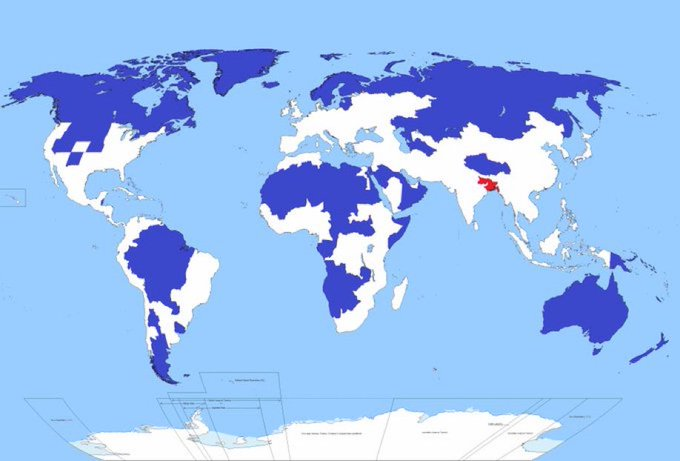
\includegraphics{fig/World_5pct_of_humans_red_blue.jpeg}

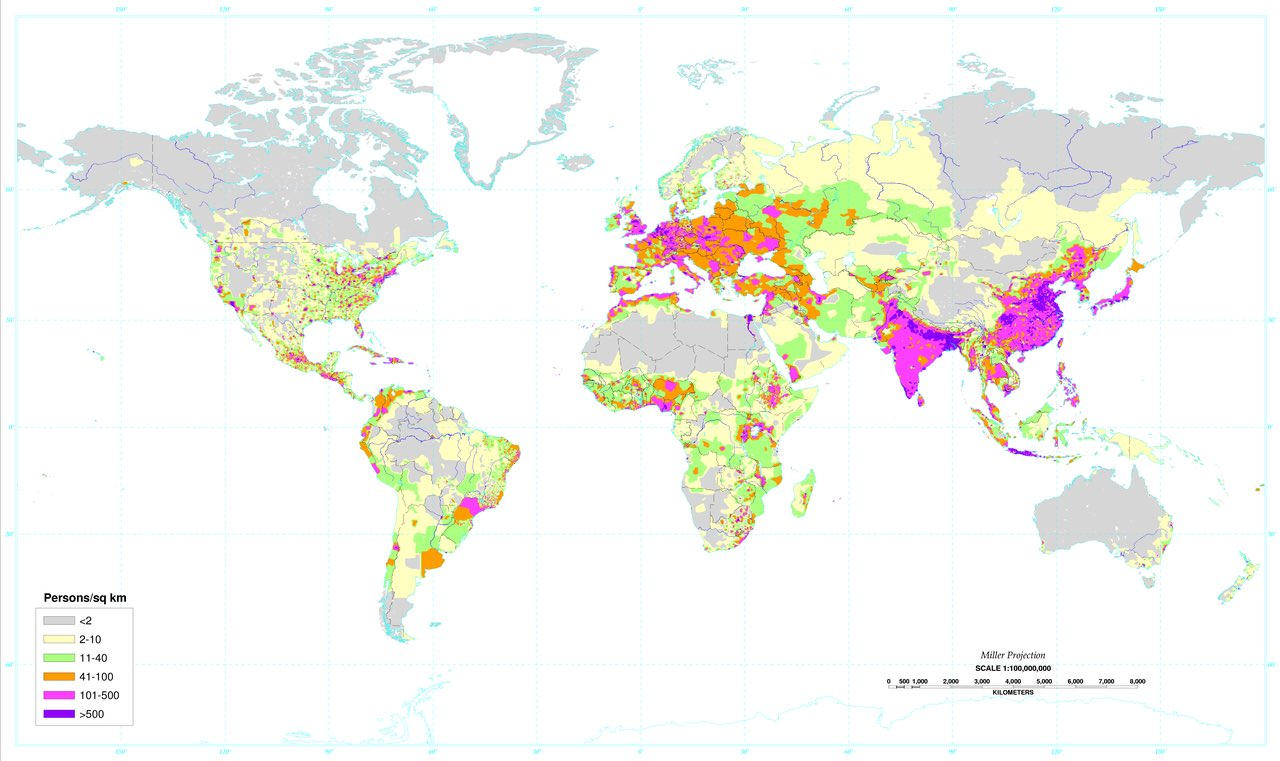
\includegraphics{fig/World_Pop_Dens_by_Color.jpeg}

\hypertarget{suburbia}{%
\chapter{Suburbia}\label{suburbia}}

Previous mainstays of suburban life are now myths: that the majority of people own their homes; that the suburbs are havens for the middle class; or that the bulk of people are young families who value privacy over urban amenities like communal spaces, walkability, and mixed-use properties.

This mismatch has led to a phenomenon called ``suburban retrofitting''.

When the suburbs are retrofitted, they can take on an astonishing array of modern issues:
car dependency, public health, supporting aging people, helping people compete for jobs,
creating water and energy resilience, and helping with social equity and justice.

\href{https://www.vice.com/en/article/y3gx5b/the-people-the-suburbs-were-built-for-are-gone}{Retrofitting Suburbia}

\hypertarget{urban-planning}{%
\chapter{Urban Planning}\label{urban-planning}}

\begin{quote}
I always hear ``It is too expensive to build nice things anymore!'' which is getting things the wrong way around: what is actually too expensive is to keep building ugly things, places off no value or no meaning, disposable buildings. Nothing is cheaper in the long run than beauty. (\citet{wrathofgnon})
\end{quote}

Urban design offers countless examples of engineering solutions gone wrong. During the last century, transportation designers responded to traffic congestion by building more roads, bigger roads, smoother roads, freeways, roundabouts, and so forth. This approach led to cities designed for cars and produced greater congestion. The engineering mindset failed to consider the deeper, systemic context.

Cars were a dubious idea in the first place, and the car culture was promoted by profiteers, not by a wise assessment of transportation options. In the 1930s, Standard Oil, General Motors, and Firestone Tire created a U.S. company, National City Lines, that bought public transportation systems and sabotaged them. They literally tore out light rail tracks and lobbied and bribed government officials around the world to build roads at public expense. Much of the world adopted a private car culture because that system benefited a few business elites, who wanted to increase profits. The engineering may have been brilliant, but the fundamental assumptions were wrong, or at least incomplete.

\href{https://mahb.stanford.edu/blog/thresholds-cascades-and-wicked-problems/}{Wicked Complexity}

\hypertarget{public-space}{%
\section{Public Space}\label{public-space}}

\emph{Barcelona}

Residences and businesses and roads will get you urbanity,
but to make a city requires public spaces --- ``the public's living room''.
(Salvador Rueda)

\emph{The American Lawn}

In the dominant American suburban model, wherein everyone lives in their own separate dwelling, there's no way to maintain vibrant public spaces --- everyone's too spread out --- so everyone basically has to recreate the benefits of public spaces in their own private estate.

The promise of the American suburban dream is that we don't need a public --- that the nuclear family can be sufficient unto itself.

The suburban dream of post-war America was that every white man could join the middle class and afford his own mini feudal estate, complete with its own stable (garage), its own compliant staff (wife and kids), and its own ornamental lawn.

We're trying to compensate for the lack of a public by accumulating more and more private stuff.
It doesn't work.

It's all so dumb. This is the thing I hate most about suburbia --- it makes the people who live in it, myself included, enthusiastic participants in their own alienation.

People need spontaneous mixing. Research shows it is the primary way humans form friendships (which is why so many professional-class Americans make lifelong friends in college, when they are forced into close proximity). The number and depth of social connections is a reliable indicator of physical health, psychological health, and longevity. Loneliness and isolation kill.

\href{https://www.volts.wtf/p/a-rant-about-lawns-in-america}{Roberts}

\hypertarget{urban-economics}{%
\chapter{Urban Economics}\label{urban-economics}}

Considering the city as an object of analysis for economists is fairly recent:
a thread on the history of US-born urban economics.

\href{https://twitter.com/Undercoverhist/status/1372999869204467718}{Beatrice Cherrier (twitter thread)}

\hypertarget{rent-gap}{%
\chapter{Rent Gap}\label{rent-gap}}

\begin{itemize}
\tightlist
\item
  Abstract Clark:*
\end{itemize}

The seeking of potential rents directs flows of investment into built and natural environments,
suffusing volatility into urban and rural landscapes, generating gentrification and other forms of
land use change, and displacing lives and livelihoods to make space for `improvement', `highest and
best use', `revitalization', or the like. In this paper we argue that potential rents are captured at
the cost of potential lives, and that rent gap theory, long central (and limited) to gentrification
theory, is more widely applicable to the dynamics of land use change and uneven geographical
development in capitalist societies. By reading David Harvey's analyses of rent and accumulation
by dispossession as a sophisticated formulation of rent gap theory, we relate the seeking and
capturing of potential rents to the power of landed developer interests and a broadened con-
ceptualization of rentiership. We furthermore relate the seeking of potential rents to an ideology
of limitless accumulation, and the striving to rein in potential rents to ideas of degrowth and the
need for a culture and a politics of limits. Brief vignettes from the `primary sector' (fisheries in the
Baltic Sea, dairy farming in Europe, and small-scale farming in Sweden) suggestively illustrate our
central argument that the seeking and capturing of potential rents stand in stark opposition to
potentials for wellbeing and flourishing of human and non-human lives. We conclude that con-
straining potential rents -- founded as they are on faith in limitless growth -- requires a culture of
self-limitation and politically imposed limitations commensurable with post-capitalist societies.

\href{pdf/Clark_2020_Rent_Gap.pdf}{Clark (2020) Potental Rents vs.~Potential Lives (pdf)}

\hypertarget{urban-research}{%
\chapter{Urban Research}\label{urban-research}}

\hypertarget{jane-jacobs}{%
\section{Jane Jacobs}\label{jane-jacobs}}

Considering her contribution to economic theory may seem counter-intuitive. In addition to lacking academic credentials, she took little interest in engaging the discipline of economics. Her models were neither formal nor developed in reference to existing models. And her view of economic theory in general was dismissive. In the opening chapter of Cities and The Wealth of Nations, ``Fool's paradise,'' Jacobs lays out a history of economic thought and arrives at this sweeping conclusion: ``Choosing among the existing schools of thought is bootless. We are on our own.'' The same dismissive stance extended to academic institutions, as she refused numerous honorary degrees from various Universities.

\textbf{Jacobs Externalities}

Some economists picked up on her insights. A type of economic externality has been derived from her detailed historical accounts of new economic activities arising from urban diversity. Chicago and Harvard urban economists \href{https://www.nber.org/papers/w3787}{Glaeser, Kallal, Scheinkman, and Shleifer credited Jacobs in 1992} for identifying cross-industry knowledge transfers, which they dubbed ``Jacobs externalities.''
The concept was based on Jacobs' The Economy of Cities and posits that knowledge transfer occur between different industries, and that local competition supports economic growth.

This came four years after future Nobel prize recipient Robert Lucas pointed to Jacobs' work while investigating the external effects of human capital in his 1988 article
\href{https://www.sciencedirect.com/science/article/abs/pii/0304393288901687}{On the Mechanics of Economic Development},
although without formalizing his insight.
Lucas' endorsement earned Jacobs increasing recognition among economists over the following decades.
Paul Krugman described her as a ``patron saint of the new growth theory'' and her unusual status
was summed up by Robert Dimand and Robert Koehn who saw her as
``her own distinctive kind of political economist \ldots{}
an exceptional instance of a woman without academic affiliation or university training
achieving recognition among leading academic economists''.
And a considerable literature grew up after Glaeser et al.'s piece.
Despite this interest in her work, extended reassessments of her contribution
to economic thought have yet to appear.

The city economy model, first developed in The Economy of Cities,argues that the desirable diversification of local economic activities depends largely on the destination of goods and services entering the city's economy. The key claim is that imports are key to economic development: they embody knowledge and allow further diversifications in the local economy, as imports are gradually replaced by local supply, and make ``room'' for new imports -- in a similar manner to import substitution. Jacobs uses this model to stress the long-term undesirability of overspecialization derived from a focus on maximizing exports, and the importance of a large and diverse local economy -- ultimately delivering a critique of comparative advantages as an organizing principle of trade.

The more niches that are filled in a given natural ecology, other things being equal,
the more efficiently it uses the energy it has at its disposal \ldots{}
That is another way of saying that economies producing diversely and amply
for their own people and producers, as well as for others,
are better off than specialized economies \ldots{}

The most elaborate study of Jacobs' use of biological and ecological analogies is provided in mathematician and philosopher David Ellerman's paper \href{http://www.ellerman.org/how-do-we-grow-jane-jacobs-on-diversification-and-specialization/}{How Do We Grow? Jane Jacobs on Diversification and Specialization (2005)}.

Depicting the city economy's boundaries as an open system governed by evolutionary dynamics:
``development is a conceptualized form of social learning.''
Incoming goods, the products of foreign know-how, are vectors of developmental learning.
And exports of commodities and services fund these imports.
When imports feed into the somewhat enclaved export economy (i.e.~overspecialized),
they have a lesser effect then when they are dissipated in local consumption.

Following Geoffrey Hodgson's taxonomy in
\href{https://www.press.umich.edu/14006/economics_and_evolution}{Economics and Evolution (1993)},
part of Jacobs' system could be characterized as phylogenetic and non-consummatory,
that is, as exhibiting an open-ended process of evolutionary selection
among a population of firms and individuals.

Jacobs targeted development schemes developed by the World Bank. She pointed to the inherent weaknesses of Robert McNamara's development strategies for addressing ``basic human needs'' (literacy, nutrition, reduction in infant mortality, and health) of poor populations. She argued that because economic development is a process, it cannot be thought of as a ``collection of things'' which can be bought or provided. The ``basic human needs approach'' ignored the necessity for solvent markets to support increased agricultural yields and the populations that were being displaced. As they could no longer rely on agricultural work to sustain themselves, displaced workers failed to find jobs in nearby city economies, where labor markets had not evolved alongside the increased agricultural yields through a succession of appropriate feedback mechanisms triggering the needed corrections. And she made the same argument against technology transfers in the ``Green Revolution'' of the 1960s and 1970s.

The mechanism of feedback relationships is one example among others of Jacobs' usage of systemic concepts to draw boundaries around the city economy as a system and elaborate on its behavior. Further examination of Jacobs' use of these concepts within the paradigm she adopted may reveal a consistent link between her analysis of cities as economic units and the policies she is tended to critique. In short, future attempts at more comprehensive interpretations of Jacobs' economic thought might benefit from stepping away from the urban focus of The Death and Life of Great American Cities while considering more carefully her later economic writings.

\href{https://hscif.org/economists-in-the-city-divry/}{Divry on Jacobs}

\hypertarget{regional-science}{%
\section{Regional Science}\label{regional-science}}

\emph{Rebours}

The history of regional science offers an interesting case study, as well as a one of the few examples, of the institutionalization of an entirely new scientific field in the years after 1945. Its foundation by Walter Isard and a group of social scientists in the 1950s represents the most institutionalized attempt to stimulate the relationship between economics and geography. The original project of Isard, who was trained as an economist at Harvard, was to promote the study of location and regional problems.

And at the outset, regional science was, in various ways, a success. It attracted many scholars from different disciplines, mostly economics, geography and urban/regional planning, and it quickly became institutionalized formally through the foundation of the Regional Science Association (RSA) in 1954 and establishment of a Regional Science Department at the University of Pennsylvania in 1958. At the same time, the creation of the Papers and Proceedings of The Regional Science Association in 1955 and of the Journal of Regional Science in 1958, offered new publication venues for scholars interested in location analysis, in particular quantitative geographers who found it difficult to publish in traditional geography journals. Within economics, regional science influenced analytical works in urban economics, as, for instance, William Alonso's thesis, widely recognized as one of the foundational works of urban economics, was written at Penn under the supervision of Isard in 1960.

However, the prevailing processes of knowledge production and evaluation which shaped the emergence of this new field were deeply influenced by economics. Geographers became dissatisfied with Isard's vision of the hierarchical division between geographers and economists, and the primacy given to economic theorizing and modelling as the core of the new regional science. Thus, the social organization of the field of regional science and its interactions with other disciplines mirrored the particularity of economics, a hierarchical discipline organized around a strong theoretical core and an insularity from the rest of social sciences.

In the late 1940s, Isard became increasingly concerned about the lack of interest among economists in the location of economic activities. His perception of the subject was not really different to his colleagues, but he wanted to improve the theory they used, which, following the British tradition of the late 19th century, suffered from a lack of spatial dimension. He did not seek to challenge the general equilibrium economic theory that was becoming dominant, but sought instead to integrate a spatial aspect within it.

In 1949 Isard was recruited to Harvard by Wassily Leontief to develop an input-output approach to regional development. During the war, input-output analysis received much attention because it enabled the American Air Force to identify the best targets for bombing. As a consequence, Leontief had received large research funds to develop his input-output framework.

Isard expressed a hierarchical division between economists, who provided
the analytical foundations of regional science,
and the geographers, who provided the empirical facts and testing.

While, the identity of economics was legitimated and reinforced by its success during the war, in geography, there was an increasing dissatisfaction with the regional geography approach that dominated the field in the1950s. The Cold War context facilitated the promotion of a new generation of quantitative geographers looking for more scientific methods.

By the mid-1970s, regional science experienced a progressive decline when geographers started to distance themselves from the analytical methods that were promoted by Isard. But even after the Regional Science Department at Penn closed its doors in 1993, regional science journals remained a going concern and continued to promote studies of spatial issues notably from urban economics and, after 1991, New Economic Geography.

\href{https://hscif.org/economists-in-the-city-rebours/}{Rebours}

\hypertarget{references}{%
\chapter{References}\label{references}}

\href{https://dyrehaugen.github.io/jdt/coronaanalysis.html}{Dyrehaugen Corona Outbreak Analysis}

\href{https://science.sciencemag.org/content/340/6139/1438}{Bettencourt (2013) Origins of Scaling in Cities}
\href{/Bettencourt_2013_Origins_of_Scaling_in_Cities.pdf}{(pdf)}
\href{/Bettencourt_2013_Origins_of_Scaling_in_Cities_SM.pdf}{(SM pdf)}

{[}Blasius (2020) Power-law distribution Covid-19{]} (\url{https://aip.scitation.org/doi/10.1063/5.0013031})
{[}(pdf){]} (/Blasius\_2020\_Power\_Law\_Covid-19.pdf)

\href{https://themes.gohugo.io/hugo-whisper-theme/}{Hugo Whisper Theme used in this Site}

\href{https://www.researchgate.net/publication/229427747_The_Statistics_of_Urban_Scaling_and_Their_Connection_to_Zipf\%27s_Law}{Gomez-Lievano (2012) Scaling Zipfs Law}
\href{/Gomez-Lievanoetal_2012_Scaling_Zipf.pdf}{(pdf)}

\href{https://www.pnas.org/content/116/28/13759}{Keuschnigg (2019) Scaling Trjectories of Cities}
\href{/Keuschnigg_2019_Scaling_Trjectories_of_Cities.pdf}{(pdf)}

\href{https://journals.plos.org/plosone/article?id=10.1371/journal.pone.0218022\#sec016}{Khiali-Miab (2019) Urban Scaling and Polycenticity Switzerland}
\href{Khiali-Miab_2019_Urban_Scaling_Polycentric_Switzerland.pdf}{(pdf)}

\href{https://www.sciencedirect.com/science/article/abs/pii/030\%204393288901687}{Lucas (1988) On the Mechanics of Economic Development}
\href{/Robert_lucas_1988_On_The_Mechanics_of_Economic_Develøopment.pdf}{(pdf)}

{[}Naik and Oldfield (2015) Urbanisation as inflicted by Capitalism{]} (\url{https://www.citymetric.com/horizons/urbanisation-not-natural-or-inevitable-its-being-inflicted-upon-us-forces-capitalism-900})

\href{https://journals.openedition.org/cybergeo/2519}{Pumain (2006) Evolutionary Theory of Urban Scaling}
\href{/Pumain_2006_Evolutionary_Theory_of_Urban_Scaling.pdf}{(pdf)}

\href{https://www.semanticscholar.org/paper/Increasing-Returns-an\%20d-Long-Run-Growth-Romer/b64575b655cf78cb97afa12eab1001a4a3959117}{Romer (1986) Increasing Returns and Long-Run Growth}
\href{/Paul_Romer_1986_Increasing_Returns_and_Long_Run_Growth.pdf}{(pdf)}

\href{https://royalsocietypublishing.org/doi/full/10.10\%2098/rsif.2013.0789}{Schläpfer (2014) Scaling of Human Interactions with City Size}
\href{/Schlapfer_2014_Scaling_Interactions_City_Size.pdf}{(pdf)}

\href{https://arxiv.org/abs/2003.10376}{Stier (2020) COVID-19 attack rate increases with citysize}
\href{/Stier_2020_COVID-19_Attcak_Rate_City_SIze.pdf}{(pdf)}

\hypertarget{part-appendices}{%
\part{Appendices}\label{part-appendices}}

\hypertarget{appendix-appendices}{%
\appendix}


\hypertarget{about}{%
\chapter{About}\label{about}}


\includegraphics{fig/me.jpg}

\emph{Dyre Haugen} and \emph{Dyrehaugen} is Webian for \emph{Jon Martin} -
self-owned Globian, Webian, Norwegian and Canarian with
a background from industrial research policy, urban planning and
economic development consulting on global, regional and urban scales.
I am deeply concerned about the (insane) way
humanity (i.e.~capitalism) interfere with nature.
In an effort to gain insights in how and why this happens
stuff is collected from around the web and put together
in a linked set of web-sites.
The sites are operated as personal notebooks.
However, these days things can be easily published to the
benefit of others concerned with the same issues.
But be aware - this is not polished for presentation or
peer-reviewed for exactness.
I offer you just to have a look at my `work-desk' as it appears in the moment.
Any comment or suggestion can be mailed to \href{mailto:dyrehaugen@gmail.com}{\nolinkurl{dyrehaugen@gmail.com}}
You can follow me on twitter as @dyrehaugen.
Thanks for visiting!

\hypertarget{links}{%
\chapter{Links}\label{links}}

\textbf{Current Dyrehaugen Sites:}

\begin{itemize}
\tightlist
\item
  \href{https://dyrehaugen.github.io/rcap}{rcap - On Capitalism} \href{http://localhost/rcap}{(loc)}
\item
  \href{https://dyrehaugen.github.io/rclm}{rclm - On Climate Change} \href{http://localhost/rclm}{(loc)}
\item
  \href{https://dyrehaugen.github.io/recs}{recs - On Economics} \href{http://localhost/recs}{(loc)}
\item
  \href{https://dyrehaugen.github.io/rngy}{rfin - On Finance} \href{http://localhost/rfin}{(loc)}
\item
  \href{https://dyrehaugen.github.io/rngy}{rngy - On Energy} \href{http://localhost/rngy}{(loc)}
\item
  \href{https://dyrehaugen.github.io/renv}{renv - On Environment} \href{http://localhost/renv}{(loc)}
\item
  \href{https://dyrehaugen.github.io/rsts}{rsts - On Statistics} \href{http://localhost/rsts}{(loc)}
\item
  \href{https://dyrehaugen.github.io/rurb}{rurb - On Urbanization} \href{http://localhost/rurb}{(loc)}
\item
  \href{https://dyrehaugen.github.io/rvar}{rvar - On Varia} \href{http://localhost/rvar}{(loc)}
\item
  \href{https://dyrehaugen.github.io/rwsd}{rwsd - On Wisdom} \href{http://localhost/rwsd}{(loc)}
\end{itemize}

\textbf{Blogs:}

\begin{itemize}
\tightlist
\item
  \href{https://dyrehaugen.github.io/rde}{rde - Blog in English} \href{http://localhost/rde}{(loc)}
\item
  \href{https://dyrehaugen.github.io/rdn}{rdn - Blog in Norwegian} \href{http://localhost/rdn}{(loc)}
\end{itemize}

\textbf{Discontinued:}

\begin{itemize}
\tightlist
\item
  \href{https://dyrehaugen.github.io/jdt}{jdt - Collection (Jekyll)} \href{http://localhost/jdt}{(loc)}
\item
  \href{https://dyrehaugen.github.io/hdt}{hdt - Collection (Hugo)} \href{http://localhost/hdt}{(loc)}
\end{itemize}

\textbf{Not listed:}

\begin{itemize}
\tightlist
\item
  (q:) dhe dhn jrw56
\item
  (z:) rcsa rpad rstart
\end{itemize}

\hypertarget{news}{%
\chapter{NEWS}\label{news}}

\hypertarget{eco-smart-singapore}{%
\section{210203 Eco-Smart Singapore}\label{eco-smart-singapore}}

In a country where over 80\% of residents live in public housing, a government commitment to sustainable urban design could have huge implications. And when it's a tropical country where convenience and air conditioning are a way of life, the impact could be greater still.

Promising 42,000 new homes across five residential districts, the eco-town of Tengah -- the Malay word for ``middle,'' though it's in the island's western region -- will be the 24th new settlement built by Singapore's government since World War II. It is, however, the first with centralized cooling, automated trash collection and a car-free town center, which conservationists hope offers a roadmap for slashing carbon emissions in the Southeast Asian city-state.

Roads, parking and utilities are being pushed beneath the town center. "We're going for the ideal concept of segregation of traffic, (with) everything underground and then the ground level totally freed up for pedestrians.

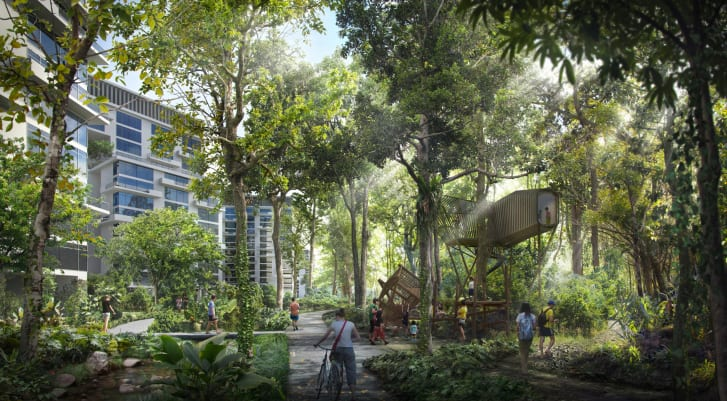
\includegraphics{fig/Singapore_Tengah_Forest_Town.jpg}

Although comparatively small, with a population of under 6 million people, Singapore's per-capita emissions are higher than those of the UK, China and neighboring Malaysia.

That's due, in part, to air conditioning, which accounts for more than a third of typical household energy consumption. Global warming will only exacerbate this dependence. The Meteorological Service Singapore (MSS) has predicted that, by the end of this century, average daily temperatures in the city-state may be at least 34.1 degrees Celsius (93.4 degrees Fahrenheit) ``almost every day'' during the eight warmest months of the year.

\emph{Centralized Cooling}
Cold water, chilled using solar power, will be piped though the district's homes, meaning residents don't need to install inefficient outdoor AC condensers (though they can still control the temperature in their own apartments).
This will generate carbon dioxide savings equivalent to taking 4,500 cars off the roads each year.

Planners used computer modeling to simulate wind flow and heat gain across the town, helping to reduce the so-called urban heat island effect.

\emph{Pneumatic Garbage Collection}
Instead of using a truck to collect garbage from every block, all the garbage will be sucked
through a pneumatic system to a chamber that serves several blocks.

\href{https://edition.cnn.com/style/article/singapore-tengah-eco-town/index.html}{Singapore building `eco smart' city (CNN)}

\hypertarget{doughnut-amsterdam}{%
\section{210125 Doughnut Amsterdam}\label{doughnut-amsterdam}}

Amsterdam Is Embracing a Radical New Economic Theory to Help Save the Environment.
Could It Also Replace Capitalism?

\begin{quote}
20th century economic thinking is not equipped to deal with the 21st century reality
\end{quote}

It's the first time a major city has attempted to put doughnut theory into action on a local level, but Amsterdam is not alone. Raworth says DEAL has received an avalanche of requests from municipal leaders and others seeking to build more resilient societies in the aftermath of COVID-19. Copenhagen's city council majority decided to follow Amsterdam's example in June, as did the Brussels region and the small city of Dunedin, New Zealand, in September, and Nanaimo, British Columbia, in December. In the U.S., Portland, Ore., is preparing to roll out its own version of the doughnut, and Austin may be close behind. The theory has won Raworth some high-profile fans; in November, Pope Francis endorsed her ``fresh thinking,'' while celebrated British naturalist Sir David Attenborough dedicated a chapter to the doughnut in his latest book, A Life on Our Planet, calling it ``our species' compass for the journey'' to a sustainable future.

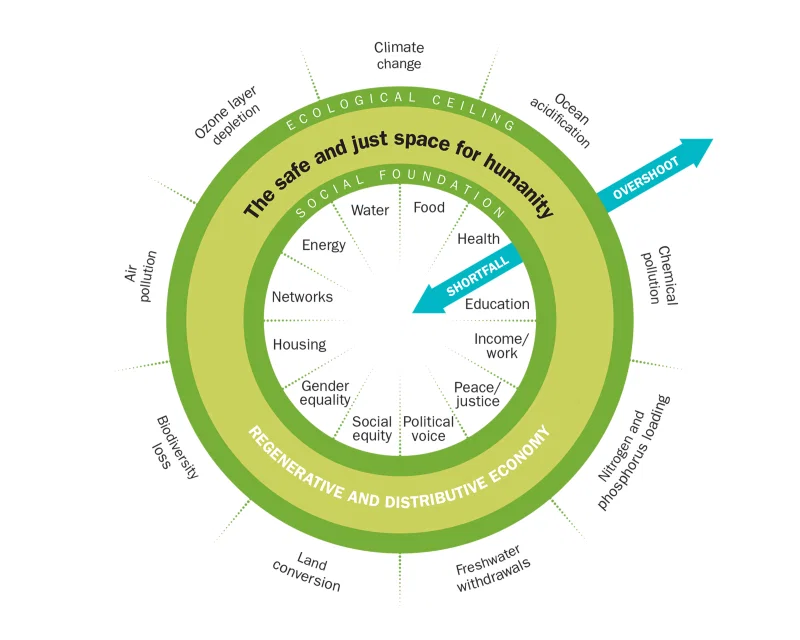
\includegraphics{fig/amsterdam-doughnut-economics-3.png}

The goal of getting ``into the doughnut'' should replace governments' and economists' pursuit of never-ending GDP growth.
The primacy of GDP overinflated when we now have many other data sets to measure economic and social well-being
Something that tries to grow endlessly we recognize as \emph{cancer}.

In 2019, C40, a network of 97 cities focused on climate action, asked Raworth to create reports on three of its members---Amsterdam, Philadelphia and Portland---showing how far they were from living inside the doughnut.

For low- and middle-income countries to climb above the doughnut's social foundation, ``significant GDP growth is very much needed.'' But that economic growth needs to be viewed as a means to reach social goals within ecological limits

Citizen-led groups focused on the doughnut that are forming in places including São Paulo, Berlin, Kuala Lumpur and California bring the potential to transform their own areas from the bottom up. ``It's powerful when you have peers inspiring peers to act.

\href{https://time.com/5930093/amsterdam-doughnut-economics/}{Doughnut Amsterdam TimeMagazin}

\hypertarget{attention-seeking-architecture}{%
\section{210125 Attention-seeking Architecture}\label{attention-seeking-architecture}}

Weird and wonderful buildings are springing up in China and elsewhere, driven by cities' desire to make a mark in a world full of eye-popping imagery.
Certain characteristics are shared, such as eye-popping imagery and curving architectural forms that stand out by virtue of being the last shapes you would come up with if you were only concerned with the practicalities of manufacture, assembly and engineering. There is the unsubtle wielding of natural and cultural symbolism -- lotus flowers, the Himalayas, silk, shanshui. There is a passion for putting trees in the air, with a correlative unconcern about whether a storeys-high planter offers a comparable experience of nature to a park on the ground. Look and shape are everything.

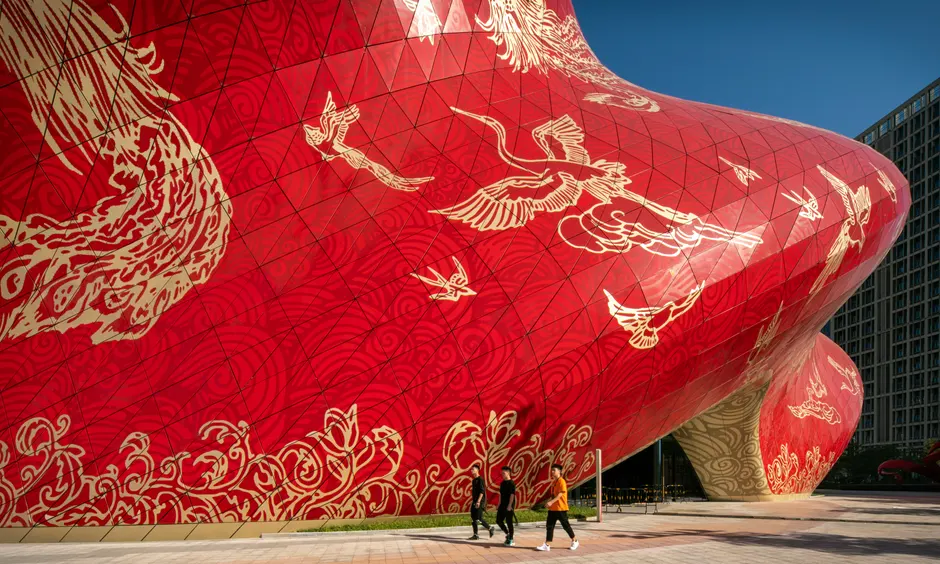
\includegraphics{fig/Sunac_Guangzhou_Grand_Theatre.png}
UrbanClick-Bait: The Sunac Guangzhou Grand Theatre - `Birthplace of the Silk Road on Sea'

The underlying factors are partly those that have always driven attention-seeking architecture, the desire of businesses and municipalities to advertise and sell themselves, the urge to make a mark, to glorify, to self-aggrandise. They are magnified by such things as (in the Arabian Gulf) the vast quantities of money available and (in China) the colossal scale at which urban developments are rolled out -- the not-small Sunac Guangzhou Grand theatre turns out to be a maraschino cherry in the vast cocktail jug of theme parks, indoor ski slopes, water rides and the like that is the Sunac Wanda cultural tourism city.

They are magnified again by technology, by the software that enables architects to visualise complex shapes and engineers to calculate them, by the photorealistic visualisation techniques that make a project seem physical before it is, by the construction techniques that turn these shapes into reality and, finally, by the internet's crowded global marketplace of imagery.

\href{https://www.theguardian.com/artanddesign/2021/jan/24/urban-clickbait-why-iconic-architecture-is-all-the-rage-again}{Guardian: Urban Click-Bait}

  \bibliography{book.bib,packages.bib}

\end{document}
